

\chapter{Assignment 2} \label{chap-3}
\textbf{Implement your own network topologies and evaluate the performance}\\
The detailed description of this assignment can be found here: \href{https://seis.bristol.ac.uk/~sy13201/DCN/Lab\%20Note.html}{Lab Note for Data Center Networking} or go to the next url: \url{https://seis.bristol.ac.uk/~sy13201/DCN/Lab\%20Note.html}


\section{Use booksim to evaluate the performance of a network topology designed in the guidance}



\subsection{Define performance metric for the evaluation}
\label{sec:3.1.1}
We will test the \textbf{latency} with different combinations of the parameters in the configuration file. (e.g., packet size, virtual channel)
    
\subsection{Results and discussion for the evaluation}

% Please add the following required packages to your document preamble:
% \usepackage[table,xcdraw]{xcolor}
% If you use beamer only pass "xcolor=table" option, i.e. \documentclass[xcolor=table]{beamer}
\begin{longtable}[H]{llllll}
\centering
\label{tab:torus_tornado}
\textbf{topology} &
  \cellcolor[HTML]{00B0F0}\textbf{\begin{tabular}[c]{@{}l@{}}injection\\ \_rate\end{tabular}} &
  \textbf{Traffic} &
  \cellcolor[HTML]{00B0F0}\textbf{\begin{tabular}[c]{@{}l@{}}packet\\ \_size\end{tabular}} &
  \cellcolor[HTML]{00B0F0}\textbf{\begin{tabular}[c]{@{}l@{}}flow\\ \_control\end{tabular}} &
  \textbf{\begin{tabular}[c]{@{}l@{}}average\\ \_packet\\ \_delay\end{tabular}} \\ \hline
\endfirsthead %以上是最前的表头
\multicolumn{6}{c}{}\\

\textbf{topology} &
  \cellcolor[HTML]{00B0F0}\textbf{\begin{tabular}[c]{@{}l@{}}injection\\ \_rate\end{tabular}} &
  \textbf{Traffic} &
  \cellcolor[HTML]{00B0F0}\textbf{\begin{tabular}[c]{@{}l@{}}packet\\ \_size\end{tabular}} &
  \cellcolor[HTML]{00B0F0}\textbf{\begin{tabular}[c]{@{}l@{}}flow\\ \_control\end{tabular}} &
  \textbf{\begin{tabular}[c]{@{}l@{}}average\\ \_packet\\ \_delay\end{tabular}} \\ \hline
\endhead %以上是换页后的表头,如未换页,并不会显示
\hline
\multicolumn{6}{r}{Continue…}\\
\endfoot %以上是前页的表尾,如未换页,并不会显示。
\hline
\endlastfoot%以上选填最后也的表尾。一般不填


testnet(r4,e3) & 0.55 & uniform & 1 & default & 9.00424 \\
testnet(r4,e3) & 0.6  & uniform & 1 & default & 9.55989 \\
testnet(r4,e3) & 0.65 & uniform & 1 & default & 11.4555 \\
testnet(r4,e3) & 0.7  & uniform & 1 & default & 15.3622 \\
testnet(r4,e3) & 0.75 & uniform & 1 & default & 36.1957 \\
testnet(r4,e3) & 0.8  & uniform & 1 & default & 50.0457 \\
testnet(r4,e3) & 0.85 & uniform & 1 & default & 87.4587 \\
testnet(r4,e3) & 0.9  & uniform & 1 & default & 114.525 \\
testnet(r4,e3) & 0.95 & uniform & 1 & default & 165.763 \\
testnet(r4,e3) & 1    & uniform & 1 & default & 209.438 \\ \hline
testnet(r4,e3) & 0.55 & uniform & 5 & default & 1035.9  \\
testnet(r4,e3) & 0.6  & uniform & 5 & default & 1178.85 \\
testnet(r4,e3) & 0.65 & uniform & 5 & default & 1303.66 \\
testnet(r4,e3) & 0.7  & uniform & 5 & default & 1452.35 \\
testnet(r4,e3) & 0.75 & uniform & 5 & default & 1569.47 \\
testnet(r4,e3) & 0.8  & uniform & 5 & default & 1714.97 \\
testnet(r4,e3) & 0.85 & uniform & 5 & default & 1842.04 \\
testnet(r4,e3) & 0.9  & uniform & 5 & default & 1966.17 \\
testnet(r4,e3) & 0.95 & uniform & 5 & default & 2091.34 \\
testnet(r4,e3) & 1    & uniform & 5 & default & 2221.98 \\ \hline
testnet(r4,e3) & 0.55 & uniform & 1 & 6       & 8.89958 \\
testnet(r4,e3) & 0.6  & uniform & 1 & 6       & 9.46639 \\
testnet(r4,e3) & 0.65 & uniform & 1 & 6       & 10.9079 \\
testnet(r4,e3) & 0.7  & uniform & 1 & 6       & 14.5966 \\
testnet(r4,e3) & 0.75 & uniform & 1 & 6       & 33.1129 \\
testnet(r4,e3) & 0.8  & uniform & 1 & 6       & 48.5042 \\
testnet(r4,e3) & 0.85 & uniform & 1 & 6       & 85.7041 \\
testnet(r4,e3) & 0.9  & uniform & 1 & 6       & 129.583 \\
testnet(r4,e3) & 0.95 & uniform & 1 & 6       & 160.373 \\
testnet(r4,e3) & 1    & uniform & 1 & 6       & 210.397 \\ \hline
testnet(r4,e3) & 0.55 & uniform & 1 & 6       & 1037.71 \\
testnet(r4,e3) & 0.6  & uniform & 1 & 6       & 1178.58 \\
testnet(r4,e3) & 0.65 & uniform & 1 & 6       & 1303.54 \\
testnet(r4,e3) & 0.7  & uniform & 1 & 6       & 1452.23 \\
testnet(r4,e3) & 0.75 & uniform & 1 & 6       & 1571.02 \\
testnet(r4,e3) & 0.8  & uniform & 1 & 6       & 1714.49 \\
testnet(r4,e3) & 0.85 & uniform & 1 & 6       & 1844.23 \\
testnet(r4,e3) & 0.9  & uniform & 1 & 6       & 1968.37 \\
testnet(r4,e3) & 0.95 & uniform & 1 & 6       & 2093.63 \\
testnet(r4,e3) & 1    & uniform & 1 & 6       & 2224.28 
\end{longtable}

\begin{figure}[H]
    \centering
    \subfigure[p1]{
    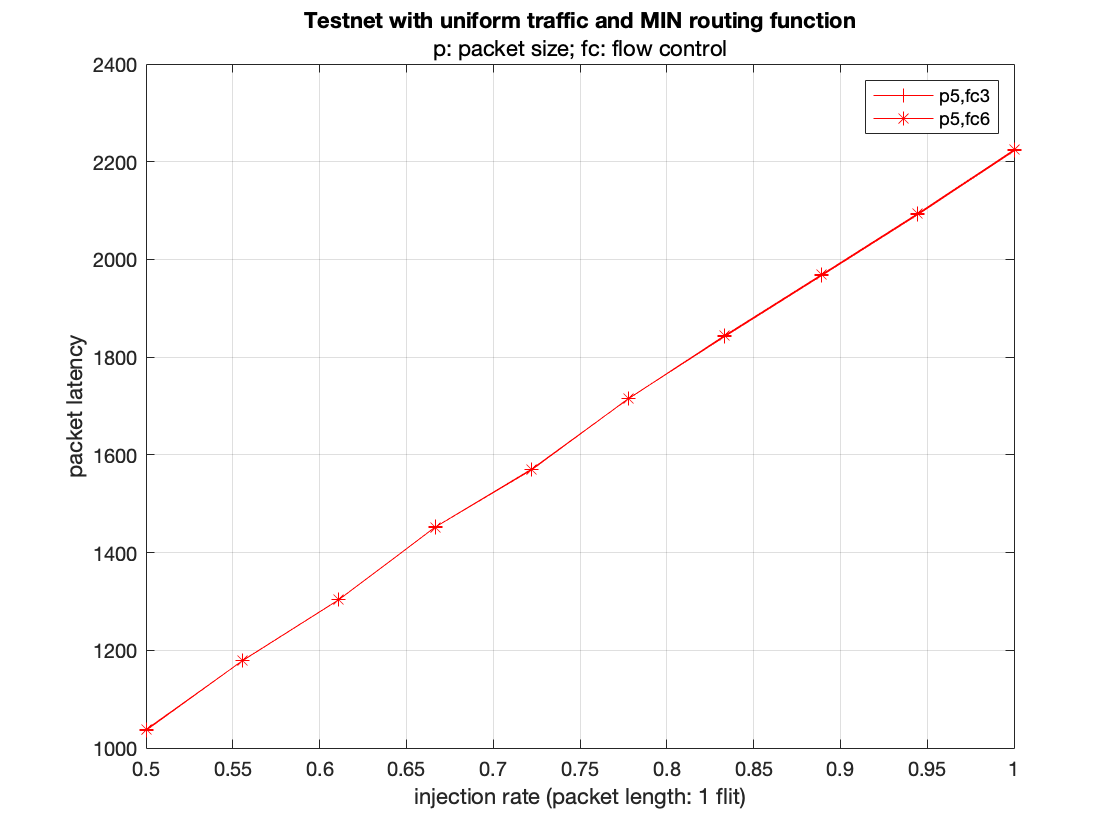
\includegraphics[width=0.45\textwidth]{Images/chap3/2_1_1.png}
    }
    \subfigure[p5]{
    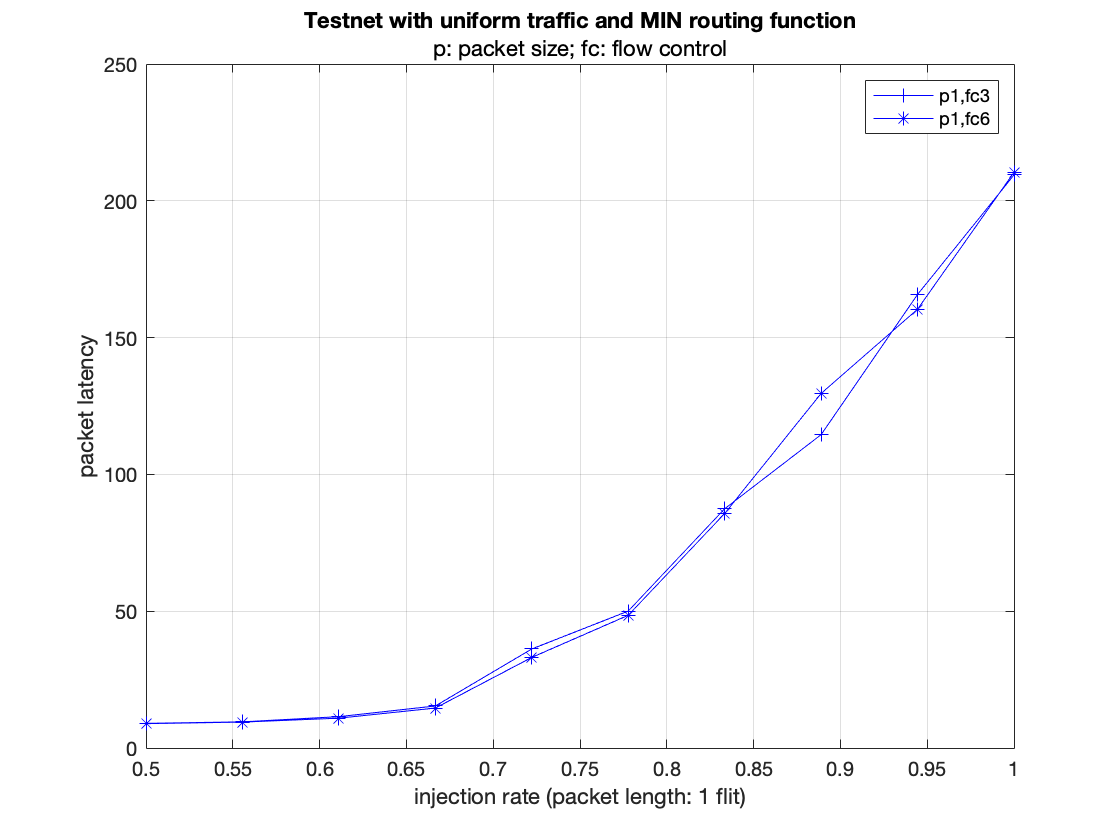
\includegraphics[width=0.45\textwidth]{Images/chap3/2_1_2.png}
    }
    \caption{Simulation results testnet}
    \label{fig:testnet_1}
\end{figure}

From Fig. \ref{fig:testnet_1}, we can find that the latency is always increasing with the increments of the injection rates. Under packet size of 1, the performances with virtual channels of 3 and 6 are almost the same. Under packet size of 5, the performances with virtual channels of 3 and 6 are slightly different.


\section{Build your own network}

\subsection{Build the network}
Build a network with the name as DesignNet. It includes 8 routers and 32 nodes. Between routers, the links drawn in the figures are bidirectional links. Here we assume a fully connected network is setup between all routers. Some links between routers are omitted for simplicity. Create the network and evaluate the performance.

% Please add the following required packages to your document preamble:
% \usepackage[table,xcdraw]{xcolor}
% If you use beamer only pass "xcolor=table" option, i.e. \documentclass[xcolor=table]{beamer}
\begin{longtable}[H]{llllll}
\centering
\label{tab:torus_tornado}
\textbf{topology} &
  \cellcolor[HTML]{00B0F0}\textbf{\begin{tabular}[c]{@{}l@{}}injection\\ \_rate\end{tabular}} &
  \textbf{Traffic} &
  \cellcolor[HTML]{00B0F0}\textbf{\begin{tabular}[c]{@{}l@{}}packet\\ \_size\end{tabular}} &
  \cellcolor[HTML]{00B0F0}\textbf{\begin{tabular}[c]{@{}l@{}}flow\\ \_control\end{tabular}} &
  \textbf{\begin{tabular}[c]{@{}l@{}}average\\ \_packet\\ \_delay\end{tabular}} \\ \hline
\endfirsthead %以上是最前的表头
\multicolumn{6}{c}{}\\

\textbf{topology} &
  \cellcolor[HTML]{00B0F0}\textbf{\begin{tabular}[c]{@{}l@{}}injection\\ \_rate\end{tabular}} &
  \textbf{Traffic} &
  \cellcolor[HTML]{00B0F0}\textbf{\begin{tabular}[c]{@{}l@{}}packet\\ \_size\end{tabular}} &
  \cellcolor[HTML]{00B0F0}\textbf{\begin{tabular}[c]{@{}l@{}}flow\\ \_control\end{tabular}} &
  \textbf{\begin{tabular}[c]{@{}l@{}}average\\ \_packet\\ \_delay\end{tabular}} \\ \hline
\endhead %以上是换页后的表头,如未换页,并不会显示
\hline
\multicolumn{6}{r}{Continue…}\\
\endfoot %以上是前页的表尾,如未换页,并不会显示。
\hline
\endlastfoot%以上选填最后也的表尾。一般不填

testnet(r4,e3) & 0.55 & uniform & 1 & default & 9.34287 \\
testnet(r4,e3) & 0.6  & uniform & 1 & default & 10.0335 \\
testnet(r4,e3) & 0.65 & uniform & 1 & default & 11.4095 \\
testnet(r4,e3) & 0.7  & uniform & 1 & default & 14.6115 \\
testnet(r4,e3) & 0.75 & uniform & 1 & default & 23.1209 \\
testnet(r4,e3) & 0.8  & uniform & 1 & default & 45.322  \\
testnet(r4,e3) & 0.85 & uniform & 1 & default & 84.0369 \\
testnet(r4,e3) & 0.9  & uniform & 1 & default & 119.761 \\
testnet(r4,e3) & 0.95 & uniform & 1 & default & 158.2   \\
testnet(r4,e3) & 1    & uniform & 1 & default & 192.858 \\
testnet(r4,e3) & 0.55 & uniform & 5 & default & 1048.03 \\
testnet(r4,e3) & 0.6  & uniform & 5 & default & 1181.38 \\
testnet(r4,e3) & 0.65 & uniform & 5 & default & 1310.65 \\
testnet(r4,e3) & 0.7  & uniform & 5 & default & 1444.5  \\
testnet(r4,e3) & 0.75 & uniform & 5 & default & 1574.2  \\
testnet(r4,e3) & 0.8  & uniform & 5 & default & 1707.99 \\
testnet(r4,e3) & 0.85 & uniform & 5 & default & 1839.84 \\
testnet(r4,e3) & 0.9  & uniform & 5 & default & 1965.54 \\
testnet(r4,e3) & 0.95 & uniform & 5 & default & 2088.24 \\
testnet(r4,e3) & 1    & uniform & 5 & default & 2218.58 \\
testnet(r4,e3) & 0.55 & uniform & 1 & 6       & 9.27776 \\
testnet(r4,e3) & 0.6  & uniform & 1 & 6       & 9.91647 \\
testnet(r4,e3) & 0.65 & uniform & 1 & 6       & 11.266  \\
testnet(r4,e3) & 0.7  & uniform & 1 & 6       & 14.5709 \\
testnet(r4,e3) & 0.75 & uniform & 1 & 6       & 22.3257 \\
testnet(r4,e3) & 0.8  & uniform & 1 & 6       & 48.0027 \\
testnet(r4,e3) & 0.85 & uniform & 1 & 6       & 89.5332 \\
testnet(r4,e3) & 0.9  & uniform & 1 & 6       & 117.538 \\
testnet(r4,e3) & 0.95 & uniform & 1 & 6       & 154.02  \\
testnet(r4,e3) & 1    & uniform & 1 & 6       & 196.502 \\
testnet(r4,e3) & 0.55 & uniform & 1 & 6       & 1048.27 \\
testnet(r4,e3) & 0.6  & uniform & 1 & 6       & 1180.26 \\
testnet(r4,e3) & 0.65 & uniform & 1 & 6       & 1309.58 \\
testnet(r4,e3) & 0.7  & uniform & 1 & 6       & 1442.91 \\
testnet(r4,e3) & 0.75 & uniform & 1 & 6       & 1576.07 \\
testnet(r4,e3) & 0.8  & uniform & 1 & 6       & 1707.35 \\
testnet(r4,e3) & 0.85 & uniform & 1 & 6       & 1840.15 \\
testnet(r4,e3) & 0.9  & uniform & 1 & 6       & 1966.2  \\
testnet(r4,e3) & 0.95 & uniform & 1 & 6       & 2088.38 \\
testnet(r4,e3) & 1    & uniform & 1 & 6       & 2218.73 \\
\end{longtable}

\begin{figure}[H]
    \centering
    \subfigure[p1]{
    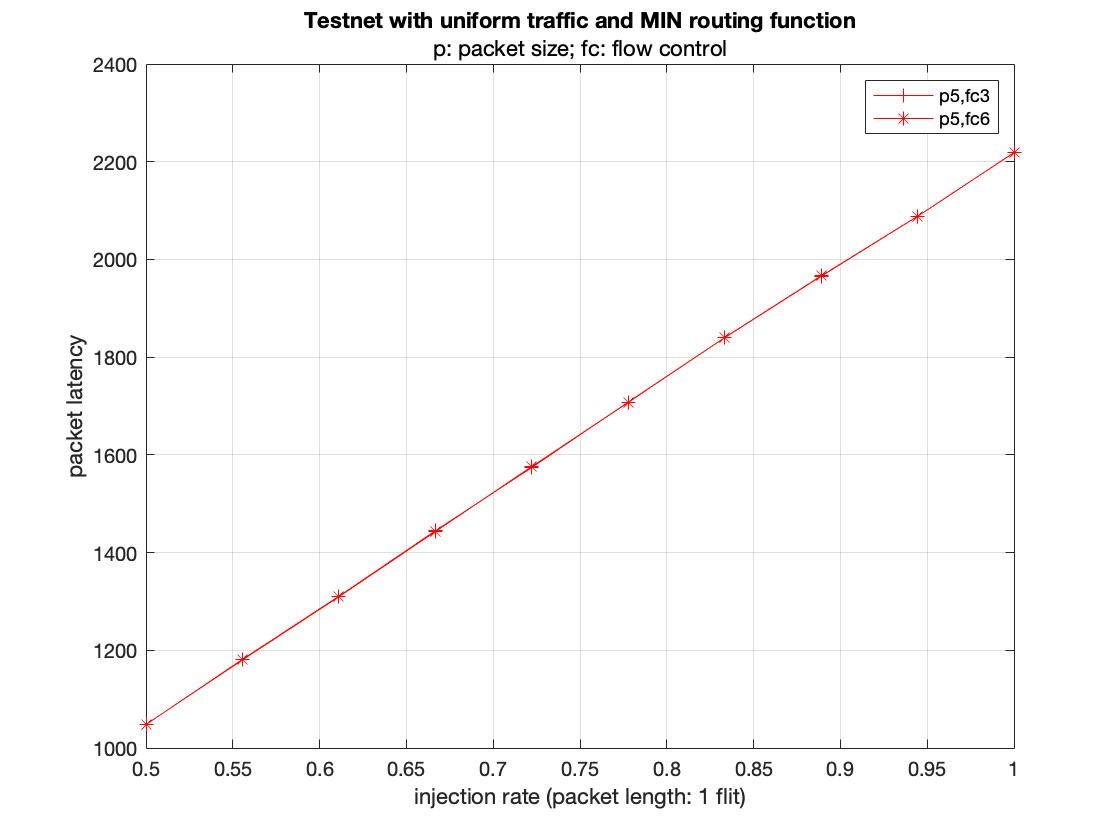
\includegraphics[width=0.45\textwidth]{Images/chap3/2_2_1.png}
    }
    \subfigure[p5]{
    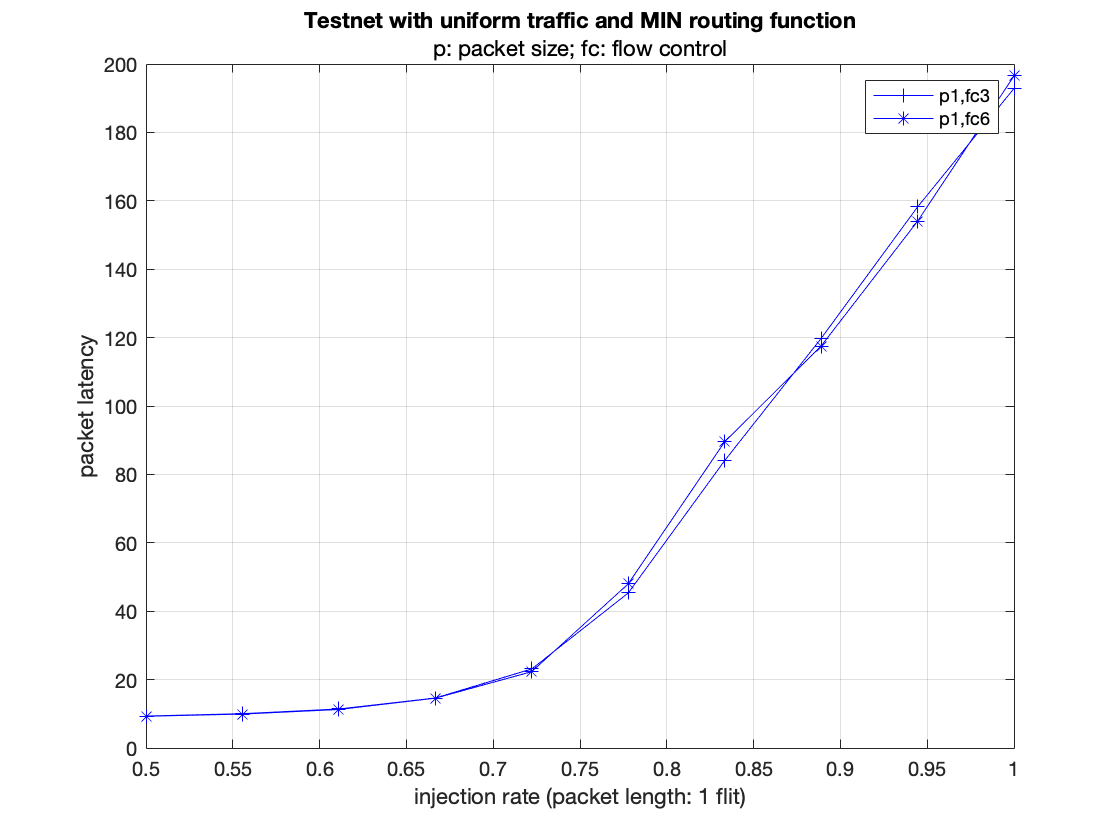
\includegraphics[width=0.45\textwidth]{Images/chap3/2_2_2.png}
    }
    \caption{Simulation results testnet}
    \label{fig:testnet_2}
\end{figure}

From Fig. \ref{fig:testnet_2}, we can find that the latency is always increasing with the increments of the injection rates. Under packet size of 1, the performances with virtual channels of 3 and 6 are almost the same. Under packet size of 5, the performances with virtual channels of 3 and 6 are slightly different.

\subsection{Evaluation}
Evaluate the performance based on the metrics defined in \ref{sec:3.1.1}.

From all the simulation results above, it is impossible to determine which routing algorithm is the best and under what kind of flow control we can get the best performance. Since the performance of a network system not only depends on the topology itself, the traffic patterns, packet size, injection rates, and flow control will all impact the performance of such a network system.

